% Copyright (c) 2017-2020 Matematyka dla Ciekawych Świata (http://ciekawi.icm.edu.pl/)
% Copyright (c) 2017-2020 Robert Ryszard Paciorek <rrp@opcode.eu.org>
% 
% MIT License
% 
% Permission is hereby granted, free of charge, to any person obtaining a copy
% of this software and associated documentation files (the "Software"), to deal
% in the Software without restriction, including without limitation the rights
% to use, copy, modify, merge, publish, distribute, sublicense, and/or sell
% copies of the Software, and to permit persons to whom the Software is
% furnished to do so, subject to the following conditions:
% 
% The above copyright notice and this permission notice shall be included in all
% copies or substantial portions of the Software.
% 
% THE SOFTWARE IS PROVIDED "AS IS", WITHOUT WARRANTY OF ANY KIND, EXPRESS OR
% IMPLIED, INCLUDING BUT NOT LIMITED TO THE WARRANTIES OF MERCHANTABILITY,
% FITNESS FOR A PARTICULAR PURPOSE AND NONINFRINGEMENT. IN NO EVENT SHALL THE
% AUTHORS OR COPYRIGHT HOLDERS BE LIABLE FOR ANY CLAIM, DAMAGES OR OTHER
% LIABILITY, WHETHER IN AN ACTION OF CONTRACT, TORT OR OTHERWISE, ARISING FROM,
% OUT OF OR IN CONNECTION WITH THE SOFTWARE OR THE USE OR OTHER DEALINGS IN THE
% SOFTWARE.

% BEGIN: System operacyjny - intro
\section{System operacyjny}

System operacyjny jest programem uruchamianym po starcie komputera (co prawda nie jako pierwszym, ale zastępującym / usuwającym z pamięci uruchomione wcześniej, więc najstarszym z działających).
% END: System operacyjny - intro

% BEGIN: Proces uruchamiania komputera
\subsection{Proces startu}

Po otrzymaniu sygnału resetu (także przy uruchamianiu systemu - "Power-on Reset") procesor po inicjalizacji rejestrów zaczyna wykonywanie kodu znajdującego się pod jakimś ustalonym adresem (typowo w wbudowanej lub zewnętrznej pamięci typu ROM lub Flash). W zależności od danej architektury / procesrora może to być m.in.: bezpośrednio kod programu użytkownika, wbudowany bootloader danego procesora umożliwiający dalsze ładowanie np. z karty SD, zewnętrzny niskopoziomowy bootloader (np. u-boot).

W przypadku architektur zgodnych z x86 jest to BIOS, który po zakończeniu procesu inicjalizacji sprzętu i testów rozruchowych ładuje do pamięci kod znajdujący się w pierwszym sektorze dysku twardego (sektorze rozruchowym rozpoczynającym się od adresu zerowego) i uruchamia go (przekazuje do niego kontrolę). Znajduje się tam kod (lub tylko początek kodu) programu rozruchowego, którego zadaniem jest załadowanie systemu operacyjnego. W przypadku współczesnych systemów linuxowych jest to zazwyczaj GRUB.

Start systemu rozpoczyna się od załadowania do pamięci obrazu jądra wraz z parametrami oraz (opcjonalnie) initrd i przekazania kontroli do jądra przez program rozruchowy (np. GRUB). W przypadku jądra linuxowego i korzystania z initrd obraz ten przekształcany jest na RAM-dysk w trybie zapisu-odczytu i montowany jako rootfs z którego uruchamiany jest \Verb#/sbin/init# (którego podstawowym zadaniem jest zamontowanie właściwego rootfs). Po jego zakończeniu (lub od razu gdy nie używamy initrd) uruchamiany jest program wskazany w opcji \Verb#init=# jądra (domyślnie typowo \Verb#/sbin/init#) z rootfs wskazanego w opcji \Verb#root=# jądra. W opcji \Verb#init=# można wskazać dowolny program lub skrypt (uruchomiony zostanie z prawami root'a).
% END: Proces uruchamiania komputera

% BEGIN: Co robi system operacyjny
\subsection{Rola systemu operacyjnego}

System operacyjny jest oprogramowaniem odpowiedzialnym za zarządzanie zasobami systemu komputerowego (sprzętem, ale nie tylko) oraz uruchomionymi na nim aplikacjami. Do najistotniejszych zadań systemu operacyjnego zalicza się podział czasu procesora i szeregowanie zadań oraz zarządzanie pamięcią - w szczególności obsługa pamięci wirtualnej, najczęściej z wykorzystaniem mechanizmu stronicowania.

Oprócz tego system zajmuje się także zarządzaniem plikami, wejściem/wyjściem (najczęściej jest ono realizowane w oparciu o przerwania (IRQ), ale znane są także modele programowego we/wy polegającego na aktywnym czekaniu), obsługą urządzeń (wejście/wyjście, sterowniki, dostęp), obsługą sieci (stos protokołów sieciowych), itd.

Współczesne systemy korzystają z co najmniej dwóch poziomów pracy - uprzywilejowanego poziomu "nadzorcy" w którym działa jądro systemu operacyjnego oraz trybu użytkownika. Operacje I/O muszą odbywać się w trybie uprzywilejowanym. Również pamięć posiada obszar chroniony, w którym umieszczany jest m.in. tablica wektorów przerwań (inaczej zmiana adresu w tym wektorze mogłaby doprowadzić do przejęcia systemu w trybie uprzywilejowanym).
% END: Co robi system operacyjny

% BEGIN: Zarządzanie procesami
\subsubsection{Zarządzanie procesami}

Jednym z głównych zadań systemu operacyjnego jest zarządzanie procesami na nim uruchomionymi - obejmuje to zarówno czynności związane z ich tworzeniem oraz kończeniem, jak też szeregowanie zadań. To system operacyjny przejmuje okresowo procesor (z użyciem przerwania zegarowego), aby podjąć decyzję (w oparciu o jakiś algorytm szeregowania zadań) który/które z porcesów gotowych do działania (czyli takich, które aktualnie nie oczekują na "coś") ma dostać przydział czasu porcesora.
% END: Zarządzanie procesami

% BEGIN: Zarządzanie pamięcią
\subsubsection{Zarządzanie pamięcią}

Drugą podstawową funkcją systemu operacyjnego, wspomnianą na początku, jest zarządzanie pamięcią. Zarządzanie pamięcią polega na odpowiednim mapowaniu adresów logicznych (używanych przez procesy) na adresy fizyczne (używane przez procesor), korzysta ono z wsparcia sprzętowego ze strony procesora.

Jest to najczęściej realizowane w oparciu o wspomniany mechanizm stronicowania. Polega to na podziale pamięci dostępnej pamięci fizycznej na jednakowe bloki zwane ramkami oraz podziale pamięci logicznej na jednakowe bloki (o tej całej wielkości co ramki) zwane stronami. Strony które są wykorzystywane przez program są mapowane na dowolne ramki pamięci fizycznej (w przypadku gdy dana strona nie zamapowana - w zależności od okoliczności błąd braku strony lub błąd ochrony strony).

\begin{center}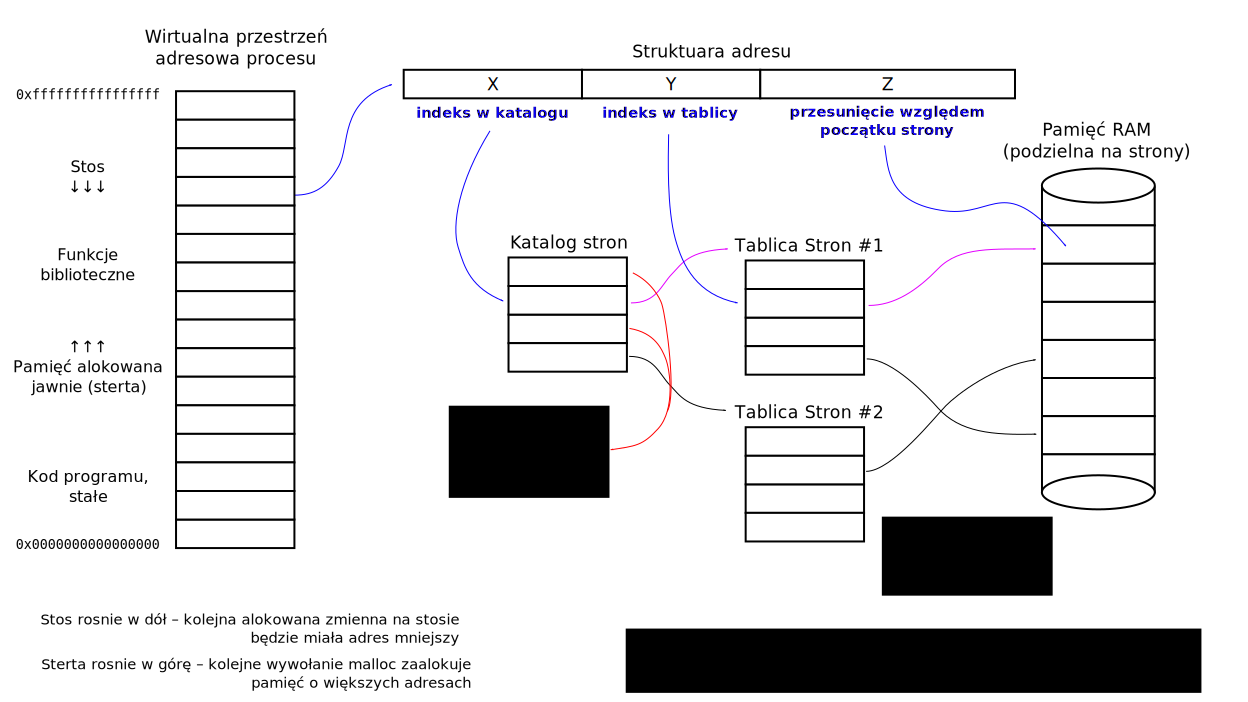
\includegraphics[width=0.95\textwidth]{img/linux/pamięć_wirtualna}\end{center}

Rozwiązuje to problem fragmentacji zewnętrznej, polegającej na braku spójnego obszaru pamięci o żądanej długości pomimo iż łączna ilość wolnej pamięci jest dostateczna, jednak nie rozwiązuje problemu fragmentacji wewnętrznej, polegającej na przydzielaniu zbyt dużych fragmentów pamięci dla procesu (a wręcz można powiedzieć że go pogłębia).

Mechanizm ten wymaga trzymania tablicy wolnych ramek, tablicy stron dla każdego procesu (zawierającej przypisania mapowań stron danego procesu na ramki) oraz wykonywania tłumaczenia adresów logicznych (strona + przesunięcie na stronie). Także sama tablica stron procesu procesu może być stronicowania (mamy tablicę która informuje nas że przypisania stron w danym zakresie adresów są przechowywane w jakiejś ramce).

Strony i ramki mogą być współdzielone pomiędzy procesami (np. przy rozgałęzianiu procesu strony są kopiowane dopiero gdy zajdzie taka potrzeba). W przypadku braku miejsca w pamięci fizycznej wybrane strony nieaktywnego aktualnie procesu mogą być umieszczane na dysku (swap).
% END: Zarządzanie pamięcią

\subsubsection{Literatura dodatkowa \zaawansowane{30}}

Było to bardzo krótkie i elementarne wprowadzenie w bardzo obszerny temat jakim są \textit{systemy operacyjne}. Wszystkich zainteresowanym niskopoziomowym działaniem systemu operacyjnego zachęcamy do zapoznania się z \href{https://pl.wikibooks.org/wiki/Pisanie_OS}{kursem pisania OS}\footnote{\url{https://pl.wikibooks.org/wiki/Pisanie_OS}} – niekoniecznie od razu pisania własnego systemu operacyjnego, ale przynajmniej zobaczeniem jak to się robi.
